\documentclass{thesisreport}
\usepackage{float}

\begin{document}

% Last modification: 2016-09-29 (Marc Deisenroth)
% Modification for UW: 2017-05-22 (jphickey)
\begin{titlepage}

\newcommand{\HRule}{\rule{\linewidth}{0.5mm}} % Defines a new command for the horizontal lines, change thickness here


%----------------------------------------------------------------------------------------
%	LOGO SECTION
%----------------------------------------------------------------------------------------



\begin{center} % Center remainder of the page

%----------------------------------------------------------------------------------------
%	HEADING SECTIONS
%----------------------------------------------------------------------------------------


\includegraphics[width = 6 cm]{./figures/ecn}\\[1.5cm] 
\textbf{\textsc{\Large Artificial Intelligence - ARTIN}}\\[1.0cm] 
\textsc{\Large École Centrale de Nantes}\\[0.5cm] 
%\textsc{\large CORO CSYS$^{1}$/ SUBJECT$^{2}$}\\[0.95cm] 

%----------------------------------------------------------------------------------------
%	TITLE SECTION
%----------------------------------------------------------------------------------------

\HRule \\[0.4cm]
{ \huge \bfseries SVM Laboratory Report}\\  % Title of your document
\HRule \\[1.5cm]
\end{center}
%----------------------------------------------------------------------------------------
%	AUTHOR SECTION
%----------------------------------------------------------------------------------------

%\begin{minipage}{0.4\hsize}
\begin{flushleft} \large
\textit{Authors:}\\
% Your name
LANCHA João\\
LOIZOU Ioannis\\
\end{flushleft}
\vspace{8cm}
\makeatletter
Date: November 29, 2023 

\vfill % Fill the rest of the page with whitespace



\makeatother


\end{titlepage}


\include{thesisfront}

\section*{Abstract}
In this laboratory, we are given the "Train cat vs non-cat" dataset and a Jupyter notebook with exercises and steps to follow. The goal of this activity is to build a simple binary classifier to distinguish images of cats and images that are not of cats based on neural networks. This is done in a two-step approach. First, we create a single-neuron model, implementing most of the functions ourselves and relying only on NumPy, to better understand the logic and how to work with neural networks. Then, we use the Keras module from TensorFlow to build a convolutional neural network (CNN).

\newpage
\newpage
\listoffigures
\listoftables
\tableofcontents

\chapter{Single Neuron Model}
For this task, we are given a dataset of 259 images of size 64x64 and 3 channels. The first step is vectorizing and splitting the data into train and test subsets (209 images for training and 50 for testing). Once the images are vectorized, each pixel now contains 3 values (1 per channel), therefore the images are vectors of size 1x12288. Figure \ref{fig:single_neuron} presents an illustration of a single-neuron neural network for a 3-dimensional input vector.

\begin{figure}[h]
  \centering
  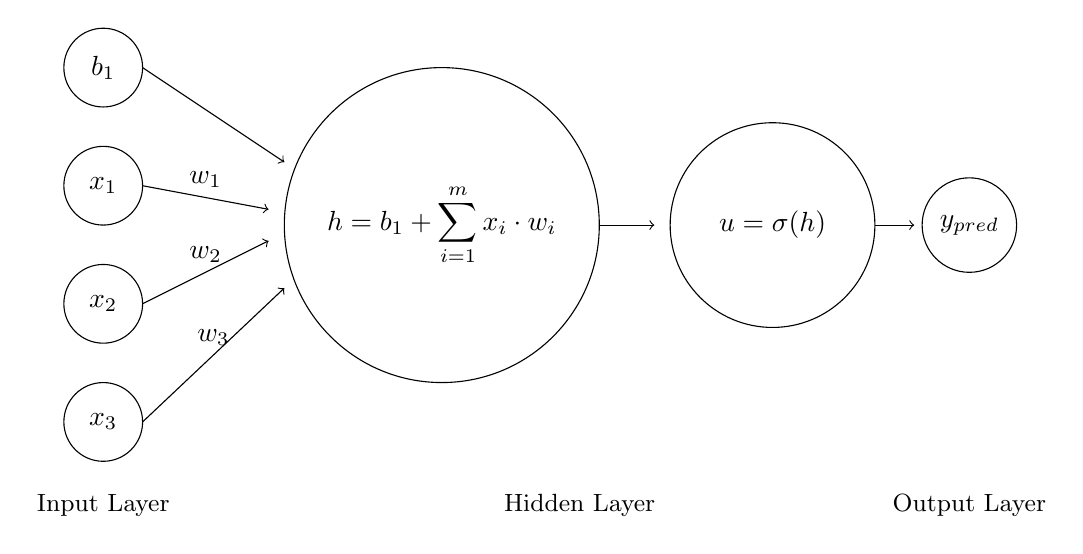
\begin{tikzpicture}
    % Inputs
    \draw (-6.5,2) circle (0.5) node[align=center] {${b}_1$};
    \draw (-6.5,0.5) circle (0.5) node[align=center] {${x}_1$};
    \draw (-6.5,-1) circle (0.5) node[align=center] {${x}_2$};
    \draw (-6.5,-2.5) circle (0.5) node[align=center] {${x}_3$};
    \node[align=center, below, font=\small] at (-6.5,-3.3) {Input Layer};
         % Arrows pointing to the central circle
        \draw[->] (-6,2) -- (-4.2,0.8);
        \draw[->] (-6,0.5) -- (-4.4, 0.2) node[midway, above] {${w}_1$};
        \draw[->] (-6,-1) -- (-4.4,-0.2) node[midway, above] {${w}_2$};
        \draw[->] (-6,-2.5) -- (-4.2,-0.8) node[midway, above] {${w}_3$};

    % Central circle
    \draw (-2.2,0) circle (2) node {$h = {b}_1 + \displaystyle\sum_{i=1}^{m} x_i \cdot w_i$};
    \node[align=center, below, font=\small] at (-0.45,-3.3) {Hidden Layer};
    \draw[->] (-0.2,0) -- (0.5,0) node[midway,above] {};

    %Activation function
    \draw (2,0) circle (1.3) node {$u = \sigma(h)$};
    
    % Output
    \draw (4.5,0) circle (0.6) node[align=center] {${y}_{pred}$};
    \node[align=center, below, font=\small] at (4.5,-3.3) {Output Layer};
    \draw[->] (3.3,0) -- (3.8,0) node[midway,above] {};  
  \end{tikzpicture}
  
  \caption{Illustration of a single neuron neural network with a 3 dimensional feature input}
  \label{fig:single_neuron}
\end{figure}


Based on the diagram in Figure \ref{fig:single_neuron}, we can clearly see the necessary steps to perform a classification with such a model.

\begin{itemize}
  \item Initialize weights ${w}_i$ and bias $b$ (we use random weight initialization and bias = 0).
  \item Define our activation function ($\sigma(x) = \frac{1}{1 + e^{-x}}$).
  \item Predict ($y_{\text{pred}} = \mathbf{w}^T \cdot \mathbf{x} + b$).
  \item Estimate the cost using binary cross-entropy loss.
\end{itemize}

Each of these steps was defined in a function in our Jupyter notebook. Next, we perform a forward pass with the help of NumPy. Everything is vectorized, so we only need 3 lines of code, calling each of the previously defined functions.

\begin{lstlisting}
w, b = initialize_parameters(train_x.shape[0])
neuron_output = neuron(w, b, train_x)
Y_pred = sigmoid(neuron_output)
\end{lstlisting}

Before the backward pass to update the weights, we need to define the compute the loss function. As previously stated, we use a binary cross-entropy loss, defined as:

\begin{equation}
E = -\frac{1}{m}\sum_{i=1}^{m} y^{(i)} \log(y_{\text{pred}}^{(i)}) + (1 - y^{(i)}) \log(1 - y_{\text{pred}}^{(i)})
\end{equation}

We then put this inside a Python function that takes as inputs the ground truths and the predictions and outputs the cost as a scalar.

Now we have everything needed to perform our backpropagation, as seen in the lectures, so we can compute the gradients of the loss function with respect to the weights and the biases. Again, this is done by declaring a Python function that takes as inputs the training set (X, Y) and the current predictions and outputs the gradients.

To calculate the gradients, we use the following definitions:

\begin{equation}
\frac{\partial E}{\partial w_i} = \frac{\mathbf{x} \cdot (\mathbf{y}_{\text{pred}} - \mathbf{y})^T}{m}
\end{equation}

\begin{equation}
\frac{\partial E}{\partial b_i} = \frac{\sum_{i=1}^{m} (y_{\text{pred}}^{(i)} - y^{(i)})}{m}
\end{equation}

We then define a function that takes as inputs the dataset, a desired number of iterations, and a learning rate and performs the gradient descent on each of the biases and weights. Using a learning rate of 0.005 over 2000 iterations, the cost had the following improvement.

\begin{figure}[H]
    \centering
    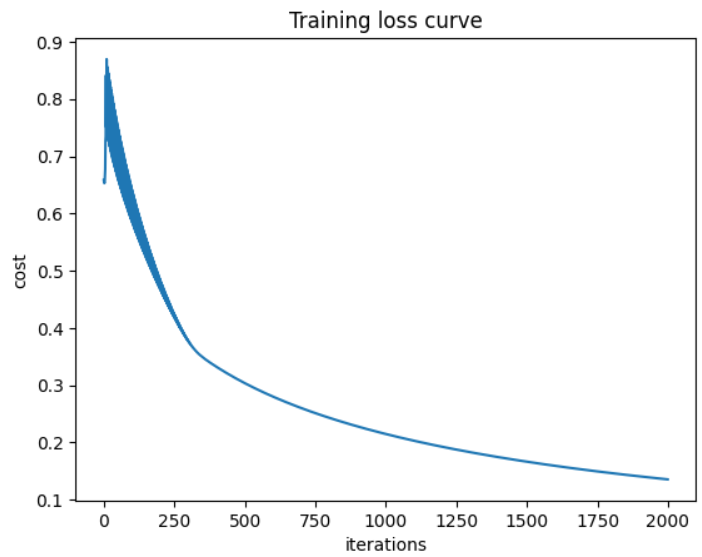
\includegraphics[width=1\linewidth]{figures/Training loss.png}
    \caption{Evolution of the loss function at each iteration of the gradient descent.}
    \label{fig:training_loss}
\end{figure}

We then predicted values using the optimized weights, which led to a training accuracy of 88.09\% and a test accuracy of 64.55\%.

However, the learning rate is a hyperparameter and, therefore, needs to be tuned. In order to successfully choose the best learning rate value, we took 10\% of the training set to use as a validation set and performed the same evaluation using 2000 iterations per learning rate, with learning rates varying from 0.001 to 0.1 with a step of 0.005, and obtained the following.

\begin{figure}[H]
    \centering
    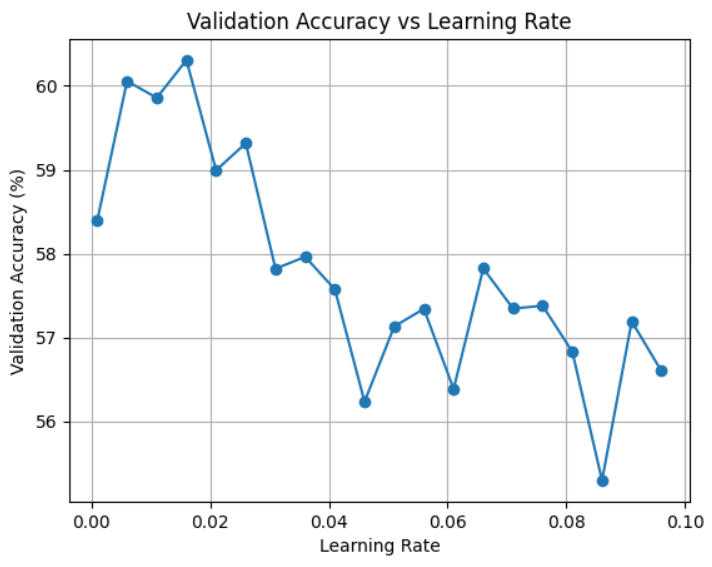
\includegraphics[width=1\linewidth]{figures/lrbest.png}
    \caption{Validation accuracy x learning rate.}
    \label{fig:lr_accuracy}
\end{figure}

Using the best-performing learning rate (0.016) from the previous step, we can introduce it to the neural network and make predictions to compare with the case where the hyperparameter was not tuned. The results are shown in the table below.

\begin{table}[H]
\centering
\begin{tabular}{|c|c|c|}
\hline
\textbf{Learning Rate} & \textbf{Training Accuracy} & \textbf{Test Accuracy} \\
\hline
0.005 & 88.09\% & 64.55\% \\
\hline
0.016 & 96.28\% & 65.54\% \\
\hline
\end{tabular}
\caption{Learning Rate and Accuracy Results}
\label{tab:learning_rates}
\end{table}
This value of learning rate is not a fixed one. Once the weights are randomly initialized, a different initialization might cause the optimal learning rate to change. As previously stated by Kinton, random weights initialization is not the best method. Instead, he proposed a pre-training step, to better initialize a NN's weights. 

\newpage

\chapter{Convolutional Neural Networks - CNNs}

\section{CNNs with Keras and Tensorflow}
After understanding the principles and implementation of a single-neuron model, we now implement a CNN, using Keras (a Google-developed API for the implementation of neural networks) and TensorFlow, a library particularly adapted to training and performance tracking of neural networks.

The first step is to adapt the example on the given link to the Keras website to work with our dataset. We make the necessary changes, such as changing the input shape that is (64x64x3), the activation function, and the loss function, among other parameters that can be seen in the Jupyter notebook. We then end up with the following model:

\begin{lstlisting}[basicstyle=\small]
model = keras.Sequential(
    [
        keras.Input(shape=input_shape), # Layer1
        layers.Conv2D(32, kernel_size=(3, 3), activation="relu"),#Layer2
        layers.MaxPooling2D(pool_size=(2,2)), # Layer 3
        layers.Conv2D(64, kernel_size=(3, 3), activation="relu"),# Layer4
        layers.MaxPooling2D(pool_size=(2,2)), # Layer5
        layers.Flatten(), # Layer6
        layers.Dropout(0.5), # Layer7
        layers.Dense(num_classes, activation="sigmoid")             
    ]
)
\end{lstlisting}

Using the \texttt{model.summary()} function, we are able to go more in-depth into our model's characteristics. It has 44,482 parameters, all of them being trainable ones, that can be broken down in the following fashion:

\begin{itemize}
  \item \textbf{Layers 2, 4, 5, and 6} do not introduce any parameters
  \item \textbf{Layer 1:} A convolutional layer with 32 3x3 filters.
    \begin{itemize}
      \item Total Parameters ($3 \times 3 \times 3 \times 32 + 1 \times 32$) = 896 Parameters;
    \end{itemize}
  \item \textbf{Layer 3:} A convolutional layer with 64 3x3 filters (input has 32 channels).
    \begin{itemize}
      \item Total Parameters ($3 \times 3 \times 32 \times 64 + 1 \times 64$) = 18,496 Parameters;
    \end{itemize}
  \item \textbf{Layer 7}: Dense ($2 \times 12544$)
    \begin{itemize}
      \item Total Parameters = 25,090 Parameters
    \end{itemize}
\end{itemize}

We then train the model with a mini-batch approach, using a batch size of 32 samples and 15 epochs, by calling the \texttt{fit()} function, which stores all the optimized weights and biases.

Afterwards, we define three other CNN architectures and train them using the same mini-batch approach. We compute the results in the ROC curve, which, as discussed in the previous report, is a very good evaluation measure to compare different classifiers.
Here are the 4 proposed architectures:\\
\begin{itemize}
  \item \textbf{Original}: The initial model adapted from the keras example
  \item \textbf{Wider}: Model with a second convolutional layer having a $5 \times 5$ kernel size.
  \item \textbf{Deeper}: One extra convolutional layer is introduced, furthermore a dropout is added between the convolutional layers, to prevent overfitting.
  \item \textbf{No pooling}: The pooling layers are removed. 
\end{itemize}

Using keras \textit{plot\_model()} function we obtain a visual representation, to better display the four architectures.

\begin{figure}[h]
  \centering
  \begin{subfigure}[b]{0.2\linewidth}
    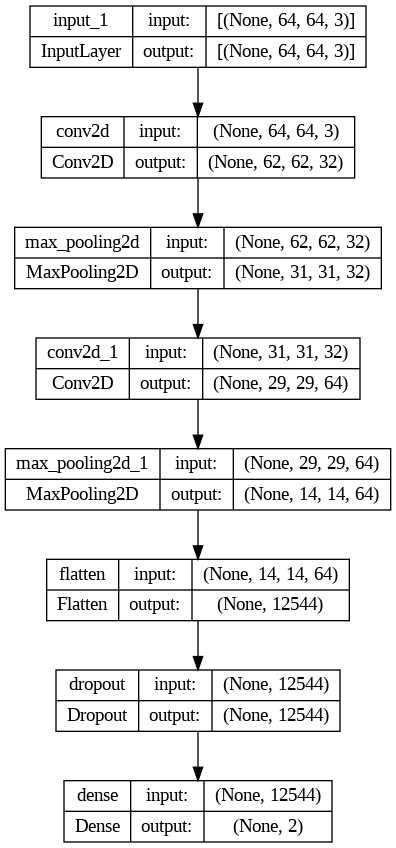
\includegraphics[width=\linewidth]{figures/original_model.png}
    \caption{Original}
  \end{subfigure}
  \begin{subfigure}[b]{0.2\linewidth}
    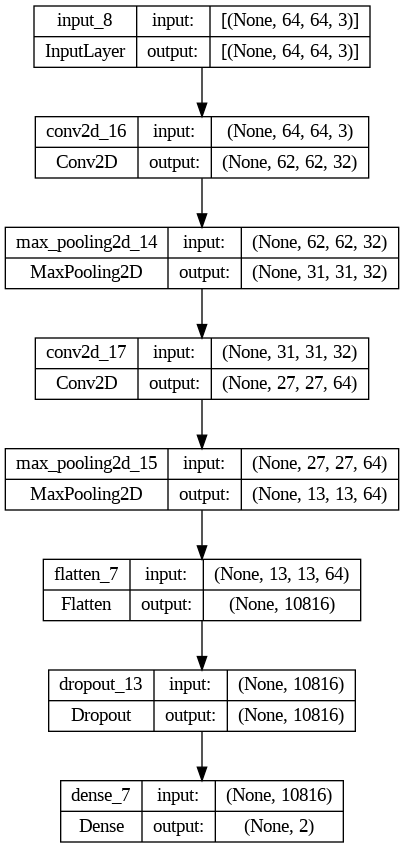
\includegraphics[width=\linewidth]{figures/model_wider.png}
    \caption{Wider}
  \end{subfigure}
  \begin{subfigure}[b]{0.2\linewidth}
    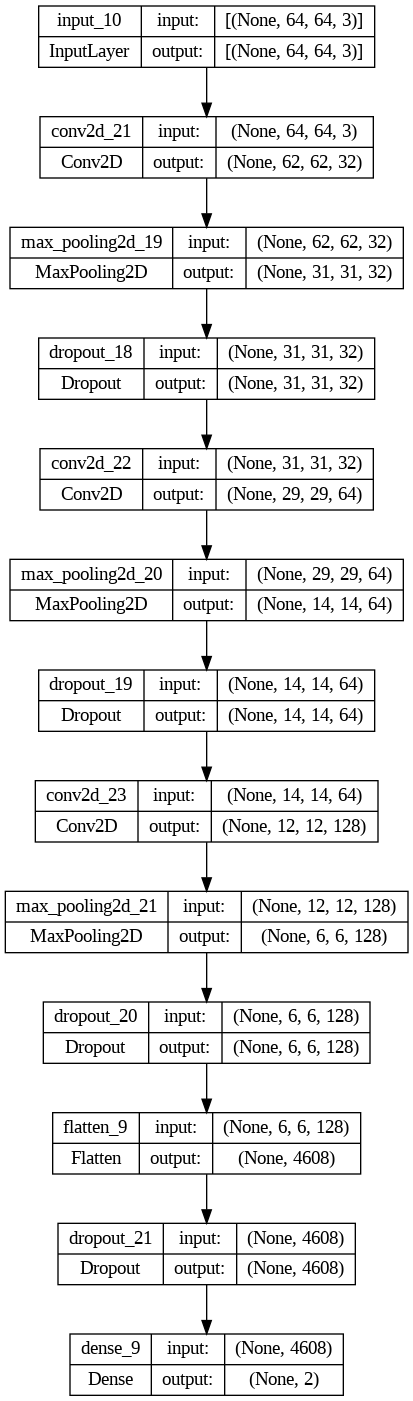
\includegraphics[width=\linewidth]{figures/model_deeper.png}
    \caption{Deeper}
  \end{subfigure}
  \begin{subfigure}[b]{0.2\linewidth}
    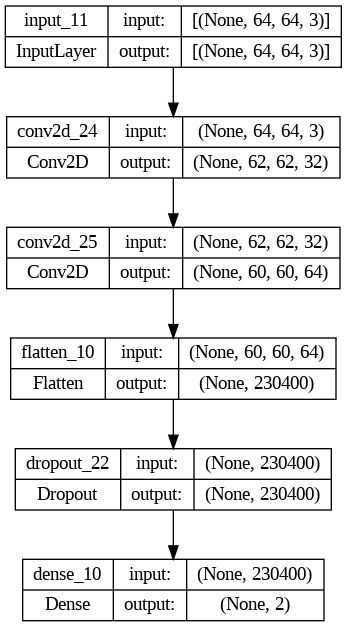
\includegraphics[width=\linewidth]{figures/model_No_pooling.png}
    \caption{No Pooling}
  \end{subfigure}
  \caption{Four architectures used }
  \label{fig:four_images}
\end{figure}


\begin{figure}[H]
    \centering
    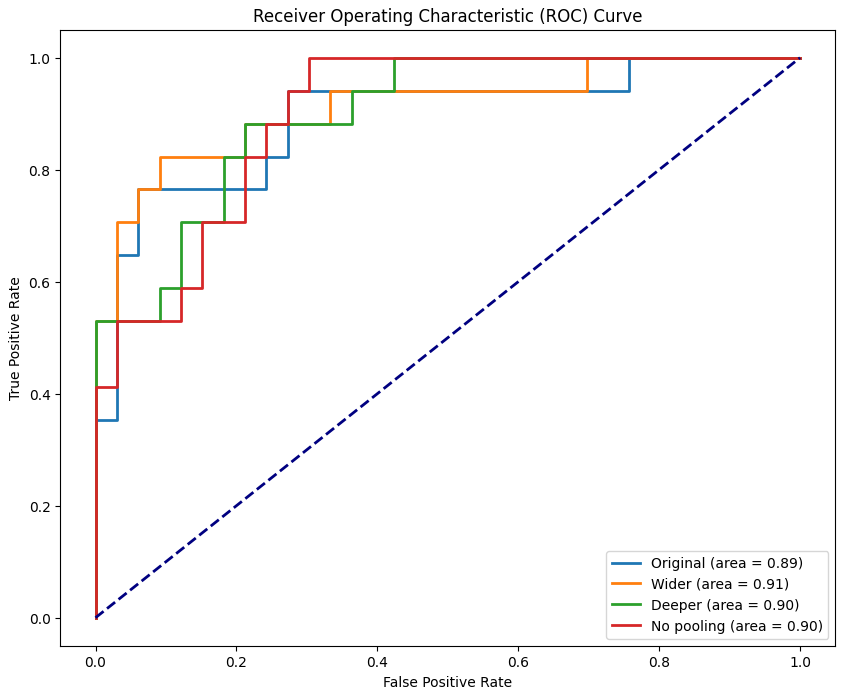
\includegraphics[width=1\linewidth]{figures/roc.png}
    \caption{ROC curves for the 4 different CNN architectures tested}
    \label{fig:lr_accuracy}
\end{figure}

\section{Custom training loop}

In this step we are asked to build our own tensorflow implementation of a training loop, to substitute the \texttt{fit()} function. The optimizer selected was 'Adam' with learning rate of 0.001. We chose Binary Cross Entropy as the loss function and a Binary Accuracy.
We introduce a callback function to allow the model to stop before the full number of epochs is completed. This is useful, once the validation loss may start to get worse, requiring an early stop to prevent overfitting.
Tensorboard was also implemented using a callback function.This allow for several parameters and relevant data from the neural network do be displayed in detail.
To code the GradCam we reccurred to the tensoflow documentation. The reason to use GradCam is to indentify which pixels are more important during the optimaztion with the gradient descent. By creating a heatmap of the picture we can clearly see which parts of the picture are more imporant for the neural network to classify the images. In our case we can clearly see in the figure below that the eyes are the most important part.
%Maybe include a graph like the one for single neuron.
%explain results
%bonus

\begin{figure}[H]
    \centering
    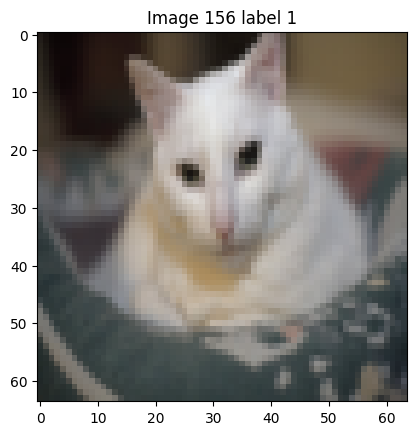
\includegraphics[width=0.5\linewidth]{figures/cat_156.png}
    \caption{The picture of a cat.}
    \label{fig:cat_156}
\end{figure}

\begin{figure}[H]
    \centering
    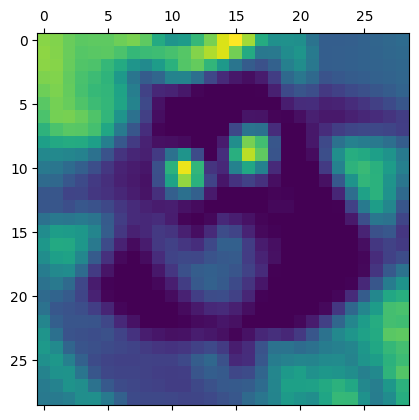
\includegraphics[width=0.5\linewidth]{figures/cat_156_heatmap.png}
    \caption{Heatmap of the picture using viridis scale.}
    \label{fig:cat_156}
\end{figure}

\newpage

\chapter*{Conclusion}
In this project, we showed how we can apply NN's and CNN's for image classification and how to improve the results. As we showed, hyperparameter tuning is an important step that should not be neglected. Otherwise, the model will not perform optimally. Additionally, neural networks are complex and powerful machine learning tools, that have thousands of possible architectures and parameters, and a good knowledge of their principles and applications is vital to correctly choose a suitable solution for a given problem. Therefore, an exercise like this, where we can test and compare different aspects of neural networks is highly enriching. 

\begin{thebibliography}{9}
  \bibitem{mateus-lecture}
    Mateus, Diana.
    \emph{Artificial Intelligence}.
    Centrale Nantes, 2023.

  \bibitem{wiki-ai}
    Wikipedia.
    \url{https://en.wikipedia.org}.

  \bibitem{scikit-learn}
    scikit-learn.
    \url{https://scikit-learn.org}.
\end{thebibliography}

\end{document}
